\documentclass[aspectratio=169]{beamer}

\usepackage[T5]{fontenc}
\usepackage[utf8]{inputenc}
\usepackage{lmodern}

\usetheme{Madrid}

\usepackage{graphicx}
\usepackage{multicol}
\usepackage{amsmath,amssymb}

% Outline look: blue text, numbered, no balls
\setbeamertemplate{section in toc}{%
  \leavevmode\inserttocsectionnumber.~\inserttocsection\par}
\setbeamercolor{section in toc}{fg=blue}

\hypersetup{colorlinks=true, urlcolor=blue}

\newcommand{\backbtn}{%
  \hfill\hyperlink{outline}{\beamerbutton{Mục lục}}}


% Giảm khoảng cách trên/dưới công thức hiển thị để slide gọn hơn
\makeatletter
\def\tight@disp{\setlength\abovedisplayskip{4pt plus 2pt}%
  \setlength\belowdisplayskip{4pt plus 2pt}%
  \setlength\abovedisplayshortskip{2pt plus 1pt}%
  \setlength\belowdisplayshortskip{2pt plus 1pt}}
\g@addto@macro\normalsize{\tight@disp}
\g@addto@macro\small{\tight@disp}
\g@addto@macro\footnotesize{\tight@disp}
\g@addto@macro\scriptsize{\tight@disp}
\makeatother

\title[Phân tích và thiết kế dầm]{Phân tích và thiết kế dầm chịu uốn}
\author[© N. V. Sỹ]{Nguyễn Văn Sỹ}
\institute[TNUT]{%
  Bộ môn Hệ thống Công nghiệp \\
  Trường Đại học Kỹ thuật Công nghiệp \\
  \href{mailto:vansy@tnut.edu.vn}{vansy@tnut.edu.vn}}
\date[Cơ học vật liệu]{\large Cơ học vật liệu – Thiết kế dầm chịu uốn \\[0.5em] \footnotesize \copyright\ Nguyễn Văn Sỹ}

\begin{document}

\begin{frame}
  \titlepage
\end{frame}
%====================
\begin{frame}{Tài liệu tham khảo}
	\small
	F. P. Beer, E. R. Johnston, Jr., J. T. DeWolf, D. F. Mazurek,
	\emph{Mechanics of Materials}, 6th ed., McGraw-Hill, New York, 2012.
	
	\vspace{1em}
	\footnotesize\color{gray}
	Toàn bộ hình vẽ trong bài giảng được trích từ giáo trình trên, chỉ sử dụng
	cho mục đích giảng dạy nội bộ.
\end{frame}
% ===== OUTLINE SLIDE =====
\begin{frame}[t]{Nội dung}
  \hypertarget{outline}{}
  \scriptsize
  \begin{multicols}{2}
    \tableofcontents[hideallsubsections]
  \end{multicols}
\end{frame}

% ===== CONTENT SLIDES =====
\section{Giới thiệu}
\begin{frame}[t]{Giới thiệu}
  \begin{columns}[T]
    \column{0.60\textwidth}
      \small
      \begin{itemize}
        \setlength{\itemsep}{0.4em}
        \item Mục tiêu: phân tích và thiết kế dầm.
        \item Dầm là các cấu kiện kết cấu chịu tải trọng tại nhiều điểm dọc
              theo chiều dài.
        \item Tải trọng ngang tác dụng lên dầm được phân loại thành tải trọng
              tập trung và tải trọng phân bố.
        \item Tải trọng tác dụng gây ra nội lực gồm một lực cắt (từ phân bố
              ứng suất tiếp) và một mô men uốn (từ phân bố ứng suất pháp).
        \item Ứng suất pháp thường là tiêu chí thiết kế quyết định:
        \[
          \sigma_x = -\frac{My}{I} \qquad
          \sigma_m = \frac{|M|c}{I} = \frac{|M|}{S}
        \]
        Cần xác định vị trí và độ lớn của mô men uốn lớn nhất.
      \end{itemize}
    \column{0.38\textwidth}
      \centering
      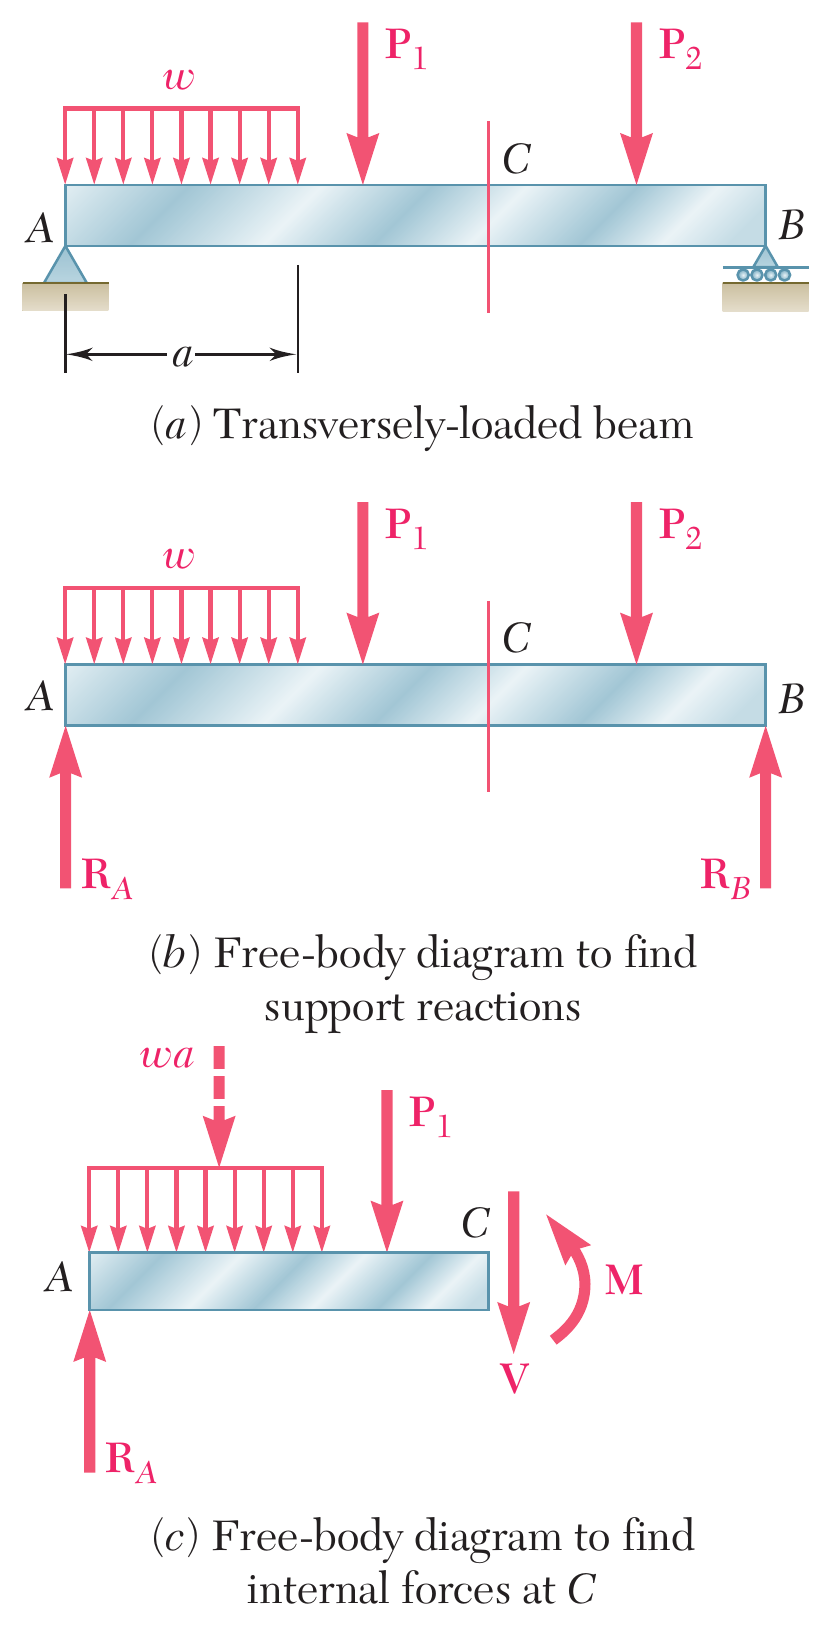
\includegraphics[width=\linewidth,height=5.5cm,keepaspectratio]{Chap_5/fig_5_4.png}
  \end{columns}
\end{frame}
% ===========
\section{Phân loại liên kết của dầm}
\begin{frame}[t]{Giới thiệu: phân loại liên kết của dầm}
  \centering
  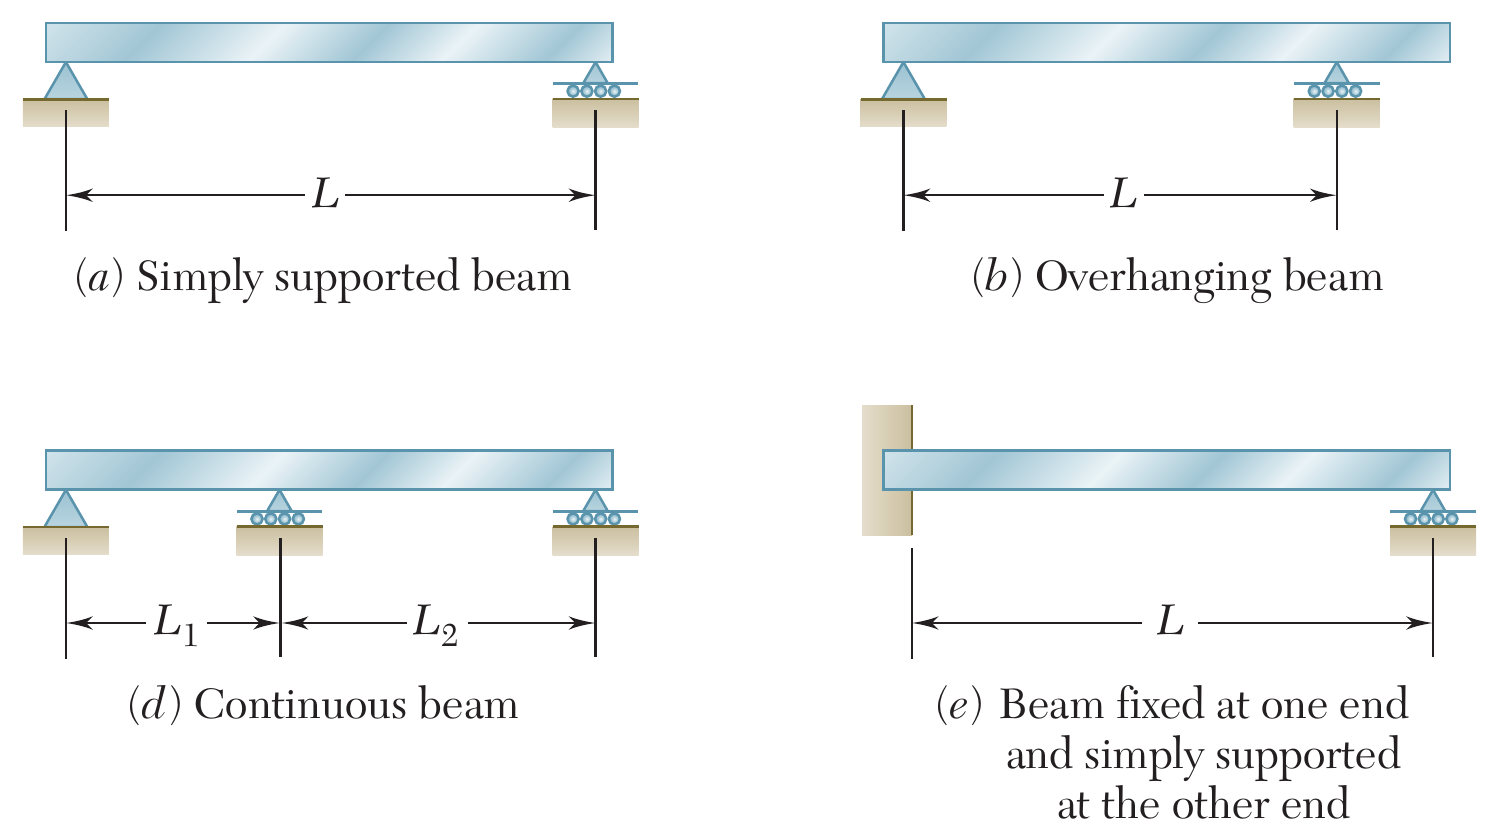
\includegraphics[width=0.9\textwidth,height=6.5cm,keepaspectratio]{Chap_5/fig_5_2.png}
\end{frame}
% ===========
\section{Biểu đồ lực cắt và mô men uốn}
\begin{frame}[t]{Biểu đồ lực cắt và mô men uốn}
  \begin{columns}[T]
    \column{0.56\textwidth}
      \small
      \begin{itemize}
        \setlength{\itemsep}{0.8em}
        \item Để xác định ứng suất pháp và ứng suất tiếp lớn nhất, cần xác
              định lực cắt và mô men uốn nội lực lớn nhất.
        \item Lực cắt và mô men uốn tại một điểm được xác định bằng cách cắt
              qua dầm tại điểm đó và phân tích cân bằng các phần dầm ở hai
              bên mặt cắt.
        \item Quy ước dấu cho lực cắt $V$, $V'$ và mô men uốn $M$, $M'$.
      \end{itemize}
    \column{0.42\textwidth}
      \centering
      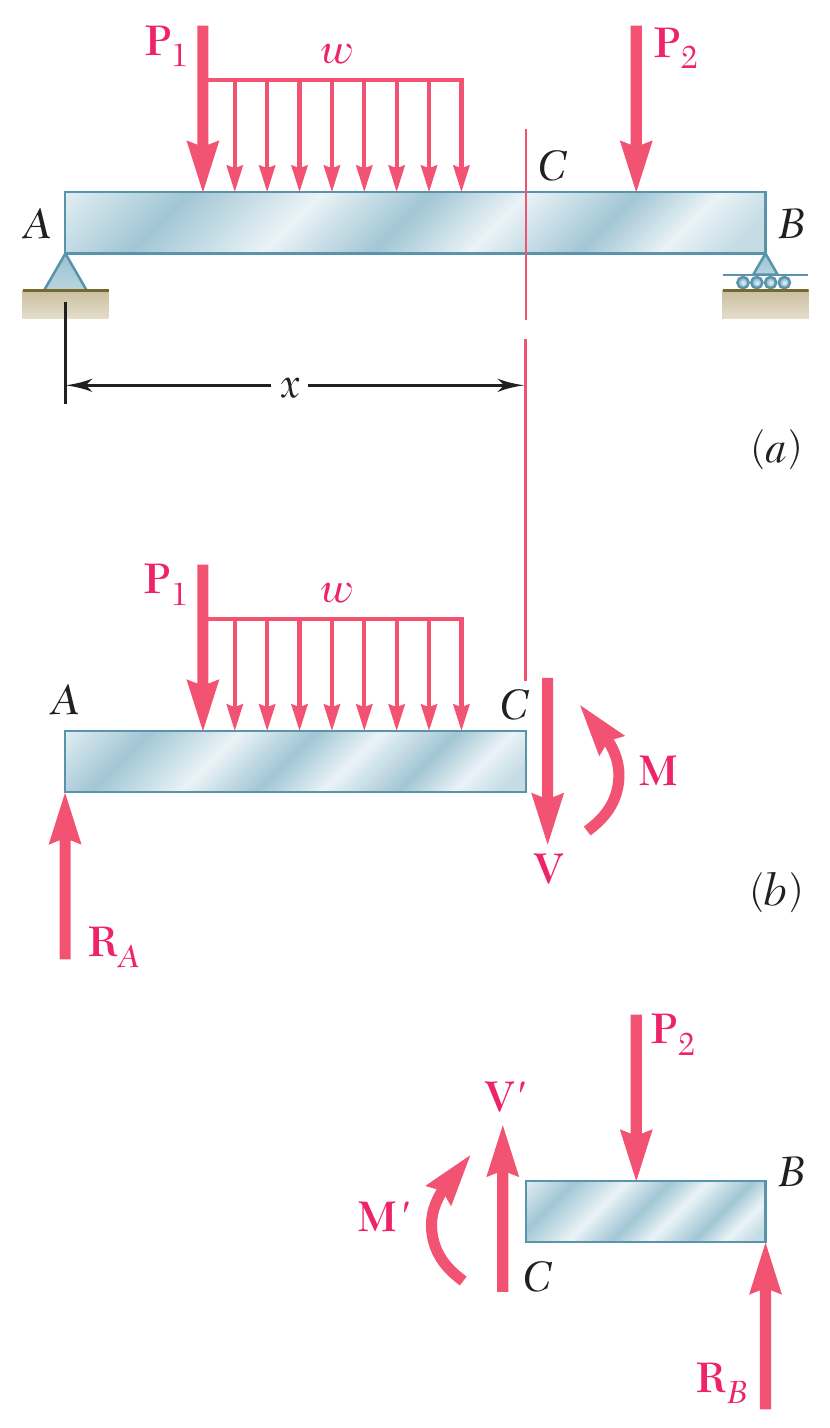
\includegraphics[width=\linewidth,height=2.9cm,keepaspectratio]{Chap_5/fig_5_5.png}\\[2pt]
      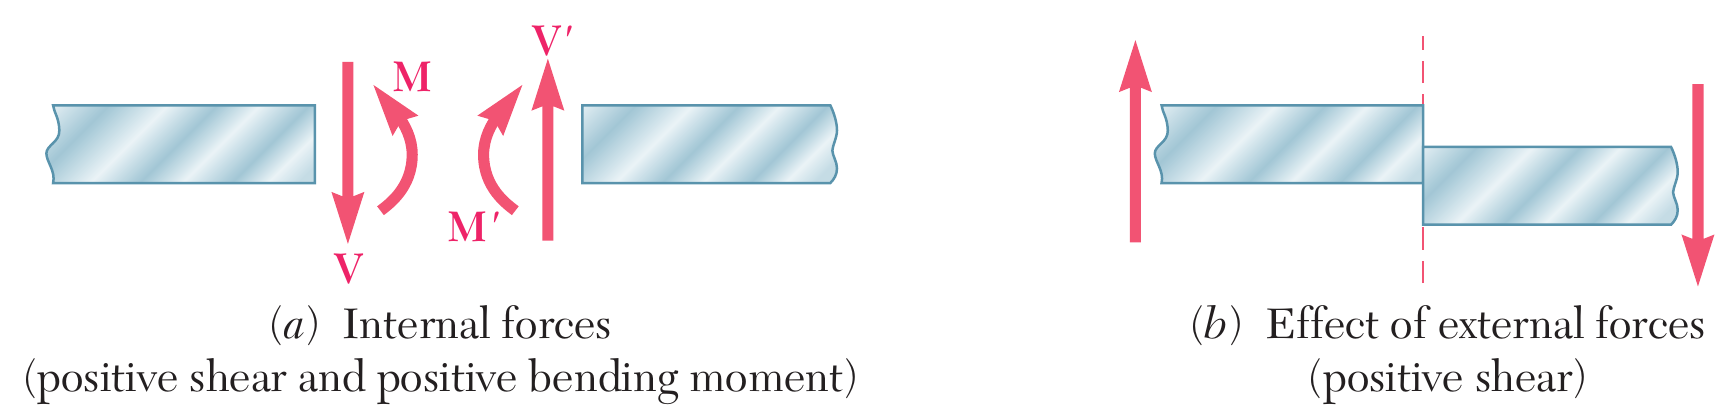
\includegraphics[width=\linewidth,height=2.9cm,keepaspectratio]{Chap_5/fig_5_6.png}
  \end{columns}
\end{frame}
% ===========
\section{Bài mẫu 5.1}
\begin{frame}[t]{Bài mẫu 5.1}
  \begin{columns}[T]
    \column{0.40\textwidth}
      \centering
      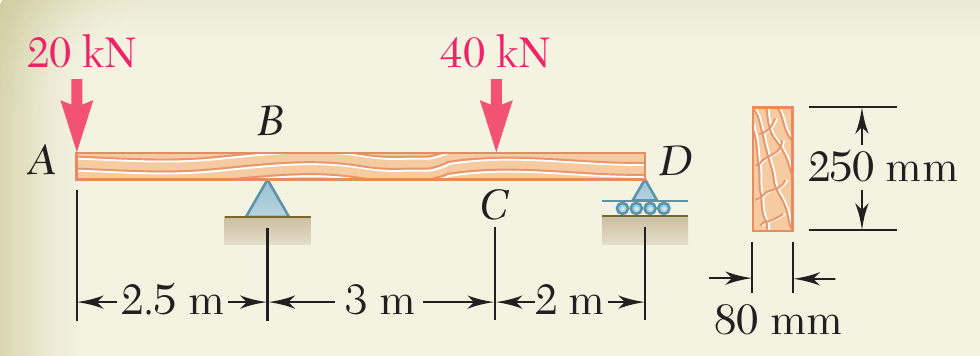
\includegraphics[width=\linewidth,height=5.5cm,keepaspectratio]{Chap_5/sp_5_1_a.png}
    \column{0.58\textwidth}
      \small
      Với dầm gỗ và tải trọng như hình vẽ, vẽ biểu đồ lực cắt và mô men
      uốn, và xác định ứng suất pháp lớn nhất do uốn.

      \vspace{0.5em}
      \textbf{LỜI GIẢI:}
      \begin{itemize}
        \setlength{\itemsep}{0.3em}
        \item Coi toàn bộ dầm là vật rắn, xác định các phản lực.
        \item Cắt dầm tại các điểm gần gối đỡ và điểm đặt lực. Phân tích cân
              bằng các phần dầm để xác định lực cắt và mô men uốn nội lực.
        \item Xác định lực cắt và mô men uốn lớn nhất từ các biểu đồ phân bố.
        \item Áp dụng công thức uốn đàn hồi để xác định ứng suất pháp lớn
              nhất tương ứng.
      \end{itemize}
  \end{columns}
\end{frame}
% ===========
\begin{frame}[t]{Bài mẫu 5.1 (tiếp)}
  \begin{columns}[T]
    \column{0.58\textwidth}
      \footnotesize
      \textbf{LỜI GIẢI:}
      \begin{itemize}
        \setlength{\itemsep}{0.3em}
        \item Coi toàn bộ dầm là vật rắn, xác định các phản lực:\\
              từ $\sum F_y = 0 = \sum M_B$: \quad
              $R_B = 46\,\mathrm{kN}$, \quad $R_D = 14\,\mathrm{kN}$
        \item Cắt dầm và phân tích cân bằng các phần dầm:
      \end{itemize}
      \[
        \begin{aligned}
          \textstyle\sum F_y &= 0: & -20\,\mathrm{kN} - V_1 &= 0 & V_1 &= -20\,\mathrm{kN}\\
          \textstyle\sum M_1 &= 0: & (20\,\mathrm{kN})(0\,\mathrm{m}) + M_1 &= 0 & M_1 &= 0\\[0.3em]
          \textstyle\sum F_y &= 0: & -20\,\mathrm{kN} - V_2 &= 0 & V_2 &= -20\,\mathrm{kN}\\
          \textstyle\sum M_2 &= 0: & (20\,\mathrm{kN})(2{,}5\,\mathrm{m}) + M_2 &= 0
              & M_2 &= -50\,\mathrm{kN\cdot m}
        \end{aligned}
      \]
      \[
        \begin{aligned}
          V_3 &= +26\,\mathrm{kN} & M_3 &= -50\,\mathrm{kN\cdot m}\\
          V_4 &= +26\,\mathrm{kN} & M_4 &= +28\,\mathrm{kN\cdot m}\\
          V_5 &= -14\,\mathrm{kN} & M_5 &= +28\,\mathrm{kN\cdot m}\\
          V_6 &= -14\,\mathrm{kN} & M_6 &= 0
        \end{aligned}
      \]
    \column{0.40\textwidth}
      \centering
      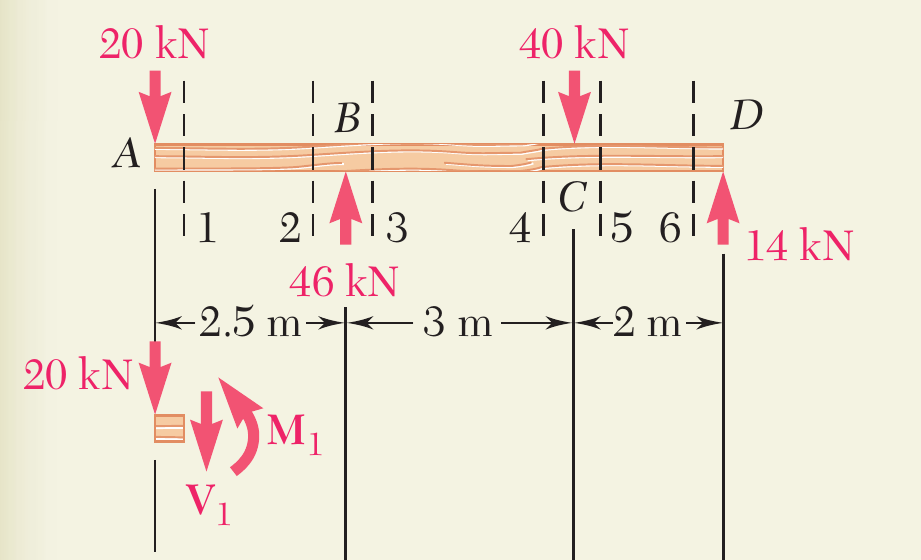
\includegraphics[width=\linewidth,height=5.5cm,keepaspectratio]{Chap_5/sp_5_1_b.png}
  \end{columns}
\end{frame}
% ===========
\begin{frame}[t]{Bài mẫu 5.1 (tiếp)}
  \begin{columns}[T]
    \column{0.56\textwidth}
      \small
      \begin{itemize}
        \setlength{\itemsep}{0.6em}
        \item Xác định lực cắt và mô men uốn lớn nhất từ các biểu đồ phân bố:
        \[
          V_m = 26\,\mathrm{kN} \qquad M_m = |M_B| = 50\,\mathrm{kN\cdot m}
        \]
        \item Áp dụng công thức uốn đàn hồi để xác định ứng suất pháp lớn
              nhất tương ứng:
        \[
          S = \tfrac{1}{6}bh^2 = \tfrac{1}{6}(0{,}080)(0{,}250)^2
            = 833{,}33\times10^{-6}\,\mathrm{m}^3
        \]
        \[
          \sigma_m = \frac{|M_B|}{S}
            = \frac{50\times10^{3}\,\mathrm{N\cdot m}}{833{,}33\times10^{-6}\,\mathrm{m}^3}
        \]
        \[
          \boxed{\sigma_m = 60{,}0\times10^{6}\,\mathrm{Pa}}
        \]
      \end{itemize}
    \column{0.42\textwidth}
      \centering
      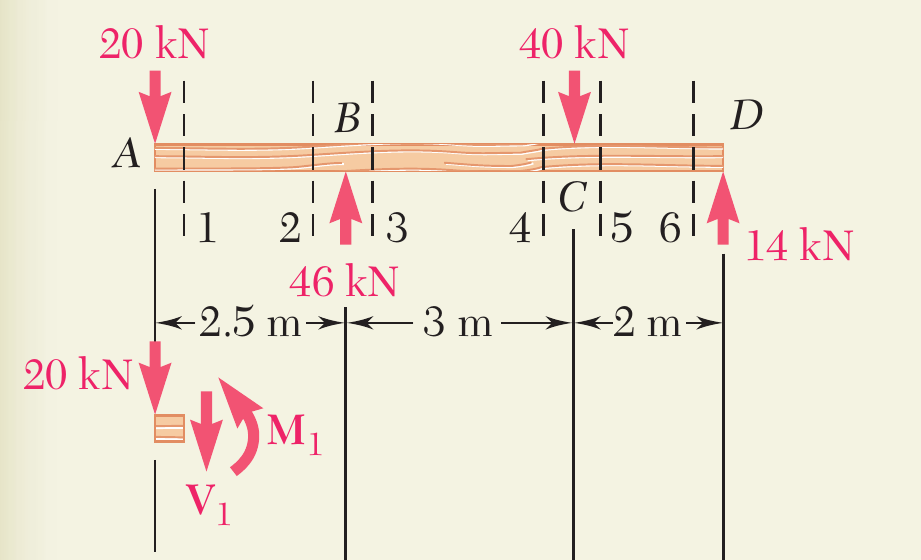
\includegraphics[width=\linewidth,height=5.5cm,keepaspectratio]{Chap_5/sp_5_1_b.png}
  \end{columns}
\end{frame}
% ===========
\section{Bài mẫu 5.2}
\begin{frame}[t]{Bài mẫu 5.2}
  \begin{columns}[T]
    \column{0.40\textwidth}
      \centering
      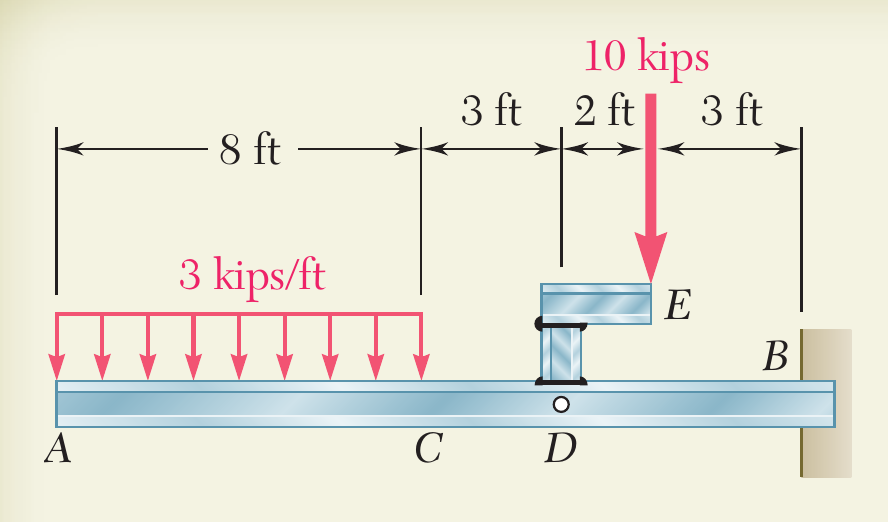
\includegraphics[width=\linewidth,height=5.5cm,keepaspectratio]{Chap_5/sp_5_2_a.png}
    \column{0.58\textwidth}
      \small
      Kết cấu như hình vẽ được làm từ dầm thép cán W250$\times$167. (a) Vẽ
      biểu đồ lực cắt và mô men uốn của dầm với tải trọng đã cho. (b) Xác
      định ứng suất pháp tại các mặt cắt ngay bên phải và bên trái điểm $D$.

      \vspace{0.5em}
      \textbf{LỜI GIẢI:}
      \begin{itemize}
        \setlength{\itemsep}{0.3em}
        \item Thay lực 45 kN bằng hệ lực -- ngẫu lực tương đương tại $D$.
              Tìm phản lực tại $B$ bằng cách coi dầm là vật rắn.
        \item Cắt dầm tại các điểm gần gối đỡ và điểm đặt lực. Phân tích cân
              bằng các phần dầm để xác định lực cắt và mô men uốn nội lực.
        \item Áp dụng công thức uốn đàn hồi để xác định ứng suất pháp lớn
              nhất bên trái và bên phải điểm $D$.
      \end{itemize}
  \end{columns}
\end{frame}
% ===========
\begin{frame}[t]{Bài mẫu 5.2 (tiếp)}
  \begin{columns}[T]
    \column{0.58\textwidth}
      \footnotesize
      \textbf{LỜI GIẢI:}
      \begin{itemize}
        \setlength{\itemsep}{0.3em}
        \item Thay lực 45 kN bằng hệ lực -- ngẫu lực tương đương tại $D$.
              Tìm phản lực tại $B$.
        \item Cắt dầm và phân tích cân bằng các phần dầm.
      \end{itemize}
      Từ $A$ đến $C$:
      \[
        \begin{aligned}
          \textstyle\sum F_y &= 0: & -45x - V &= 0 & V &= -45x\,\mathrm{kN}\\
          \textstyle\sum M_1 &= 0: & (45x)\left(\tfrac{1}{2}x\right) + M &= 0
              & M &= -22{,}5x^2\,\mathrm{kN\cdot m}
        \end{aligned}
      \]
      Từ $C$ đến $D$:
      \[
        \begin{aligned}
          \textstyle\sum F_y &= 0: & -108 - V &= 0 & V &= -108\,\mathrm{kN}\\
          \textstyle\sum M_2 &= 0: & 108(x - 1{,}2) + M &= 0
              & M &= (129{,}6 - 108x)\,\mathrm{kN\cdot m}
        \end{aligned}
      \]
      Từ $D$ đến $B$:
      \[
        V = -153\,\mathrm{kN} \qquad M = (305{,}1 - 153x)\,\mathrm{kN\cdot m}
      \]
    \column{0.40\textwidth}
      \centering
      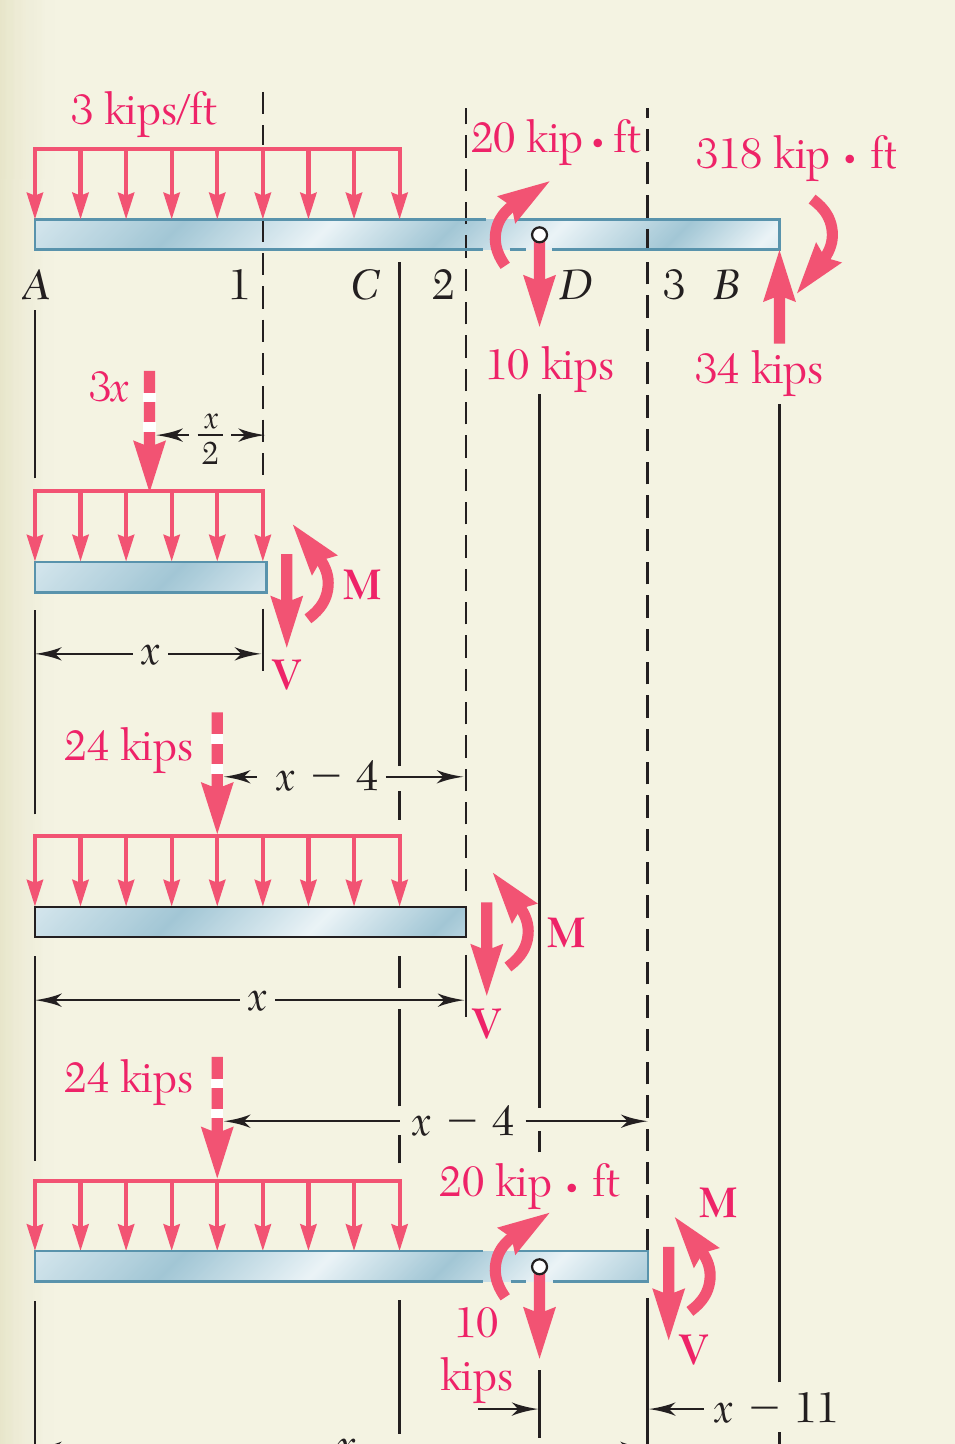
\includegraphics[width=\linewidth,height=5.5cm,keepaspectratio]{Chap_5/sp_5_2_b.png}
  \end{columns}
\end{frame}
% ===========
\begin{frame}[t]{Bài mẫu 5.2 (tiếp)}
  \begin{columns}[T]
    \column{0.56\textwidth}
      \small
      \begin{itemize}
        \setlength{\itemsep}{0.6em}
        \item Áp dụng công thức uốn đàn hồi để xác định ứng suất pháp lớn
              nhất bên trái và bên phải điểm $D$.
      \end{itemize}
      Từ Phụ lục C, với thép hình W250$\times$167,
      $S = 2{,}08\times10^{-3}\,\mathrm{m}^3$ đối với trục X--X.

      \vspace{0.5em}
      Bên trái $D$:
      \[
        \sigma_m = \frac{|M|}{S}
          = \frac{226{,}8\times10^{3}\,\mathrm{N\cdot m}}{2{,}08\times10^{-3}\,\mathrm{m}^3}
        \qquad \boxed{\sigma_m = 109\,\mathrm{MPa}}
      \]
      Bên phải $D$:
      \[
        \sigma_m = \frac{|M|}{S}
          = \frac{199{,}8\times10^{3}\,\mathrm{N\cdot m}}{2{,}08\times10^{-3}\,\mathrm{m}^3}
        \qquad \boxed{\sigma_m = 96\,\mathrm{MPa}}
      \]
    \column{0.42\textwidth}
      \centering
      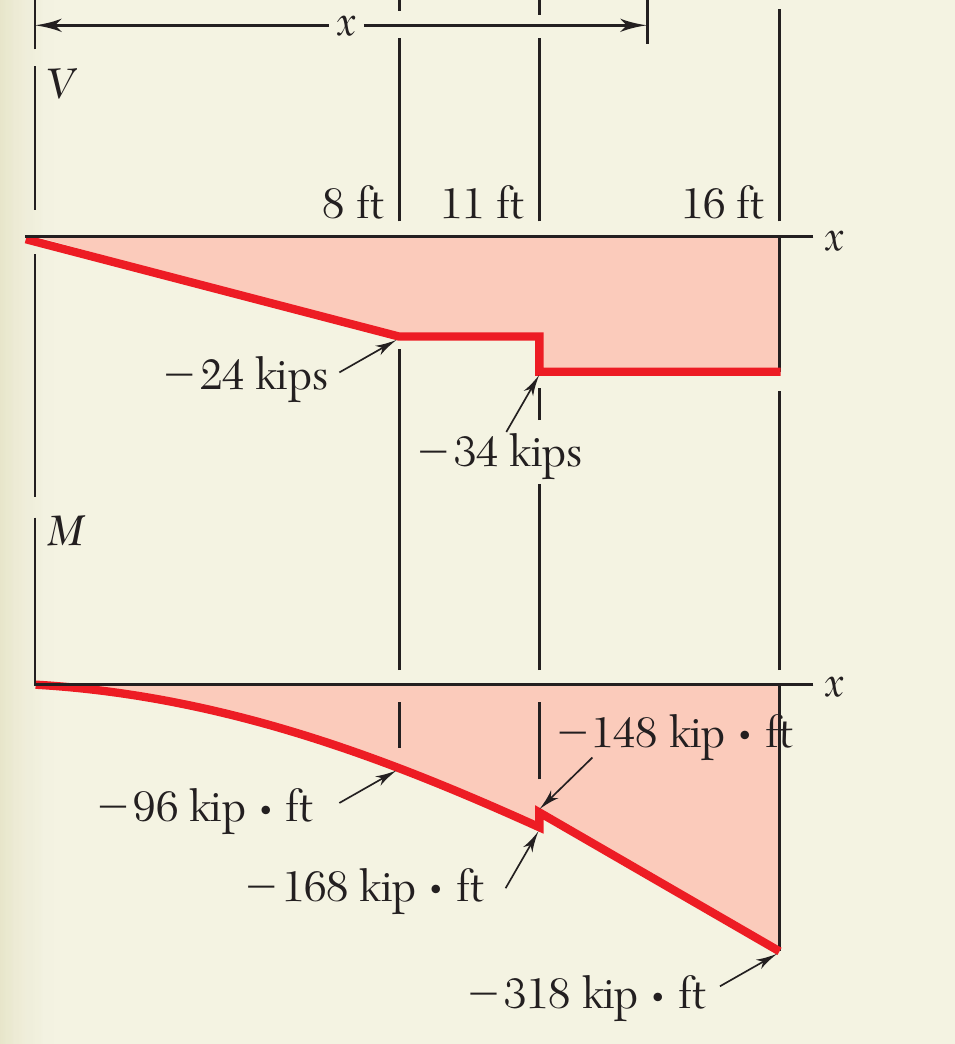
\includegraphics[width=\linewidth,height=5.5cm,keepaspectratio]{Chap_5/sp_5_2_c.png}
  \end{columns}
\end{frame}
% ===========
\section{Quan hệ giữa tải trọng, lực cắt và mô men uốn}
\begin{frame}[t]{Quan hệ giữa tải trọng, lực cắt và mô men uốn}
  \begin{columns}[T]
    \column{0.60\textwidth}
      \footnotesize
      \begin{itemize}
        \setlength{\itemsep}{0.4em}
        \item Quan hệ giữa tải trọng và lực cắt:
        \[
          \textstyle\sum F_y = 0: \quad V - (V + \Delta V) - w\Delta x = 0
        \]
        \[
          \Delta V = -w\Delta x \qquad \frac{dV}{dx} = -w
        \]
        \[
          V_D - V_C = -\int_{x_C}^{x_D} w\,dx
        \]
        \item Quan hệ giữa lực cắt và mô men uốn:
        \[
          \textstyle\sum M_{C'} = 0: \quad
          (M + \Delta M) - M - V\Delta x + w\Delta x\frac{\Delta x}{2} = 0
        \]
        \[
          \Delta M = V\Delta x - \tfrac{1}{2}w(\Delta x)^2 \qquad
          \frac{dM}{dx} = V
        \]
        \[
          M_D - M_C = \int_{x_C}^{x_D} V\,dx
        \]
      \end{itemize}
    \column{0.38\textwidth}
      \centering
      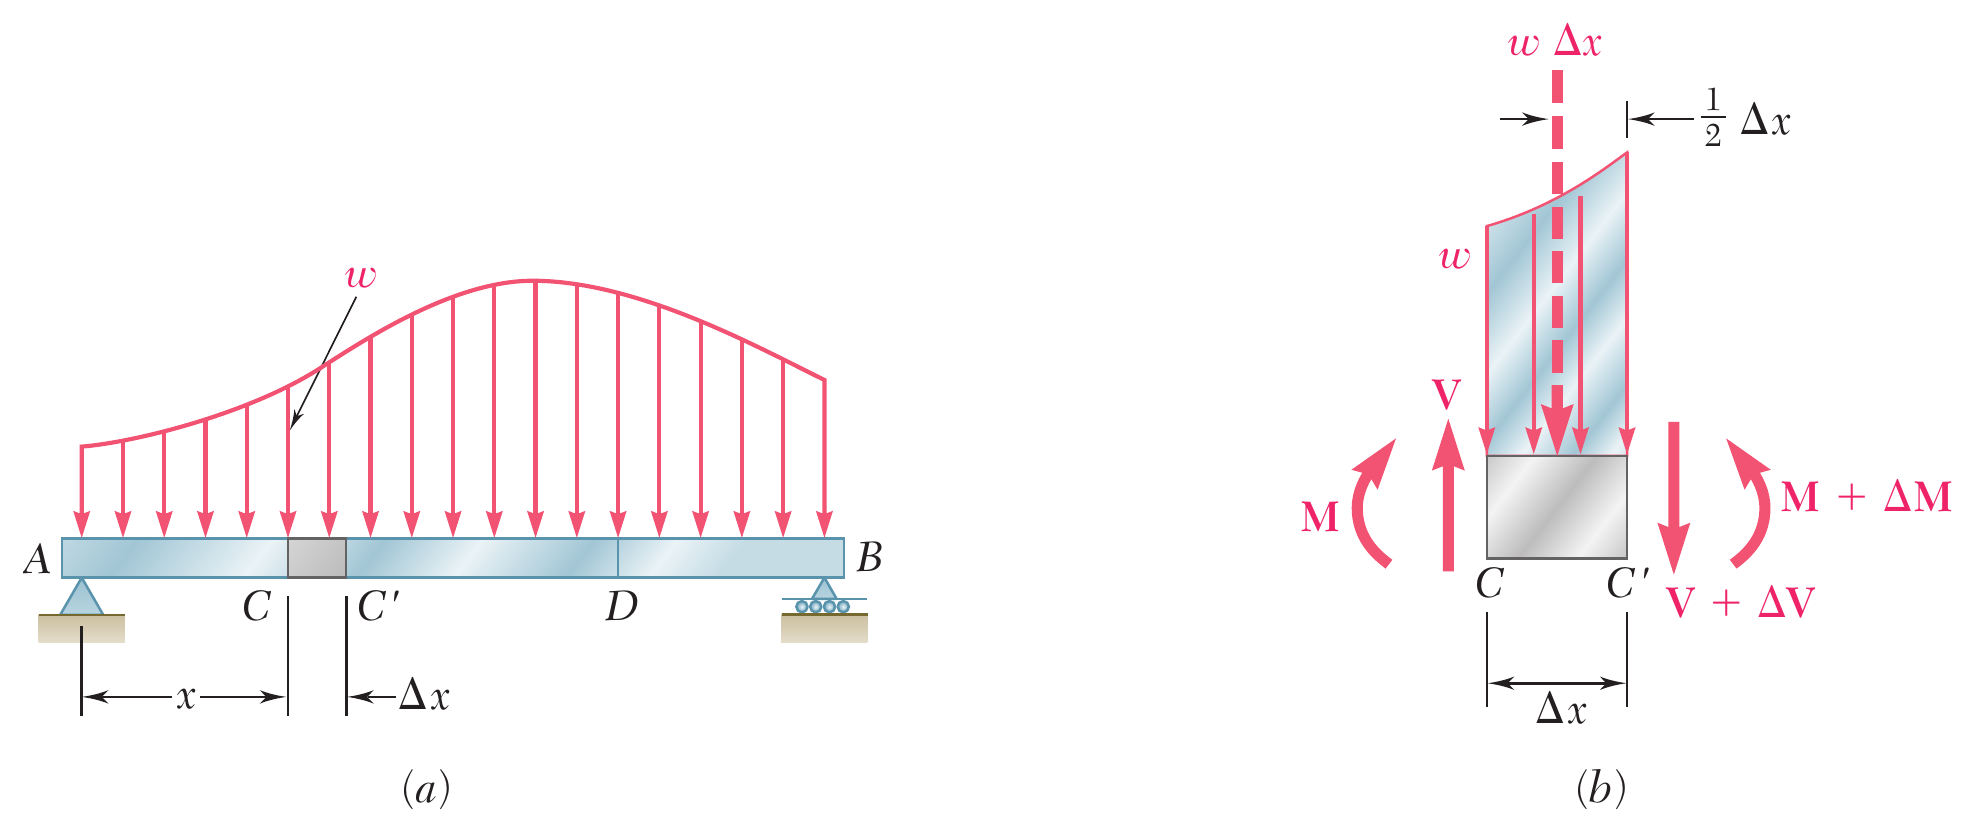
\includegraphics[width=\linewidth,height=5.5cm,keepaspectratio]{Chap_5/fig_5_11.png}
  \end{columns}
\end{frame}
% ===========
\section{Bài mẫu 5.3}
\begin{frame}[t]{Bài mẫu 5.3}
  \begin{columns}[T]
    \column{0.44\textwidth}
      \centering
      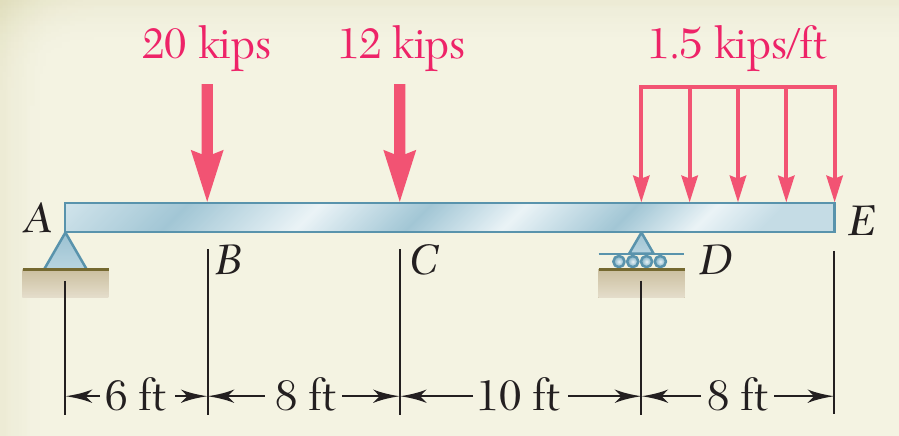
\includegraphics[width=\linewidth,height=5.5cm,keepaspectratio]{Chap_5/sp_5_3_a.png}
    \column{0.54\textwidth}
      \small
      Vẽ biểu đồ lực cắt và mô men uốn cho dầm và tải trọng như hình vẽ.

      \vspace{0.8em}
      \textbf{LỜI GIẢI:}
      \begin{itemize}
        \setlength{\itemsep}{0.6em}
        \item Coi toàn bộ dầm là vật thể tự do, xác định phản lực tại $A$ và
              $D$.
        \item Áp dụng quan hệ giữa lực cắt và tải trọng để vẽ biểu đồ lực
              cắt.
        \item Áp dụng quan hệ giữa mô men uốn và lực cắt để vẽ biểu đồ mô men
              uốn.
      \end{itemize}
  \end{columns}
\end{frame}
% ===========
\begin{frame}[t]{Bài mẫu 5.3 (tiếp)}
  \begin{columns}[T]
    \column{0.58\textwidth}
      \scriptsize
      \textbf{LỜI GIẢI:}
      \begin{itemize}
        \setlength{\itemsep}{0.20em}
        \item Coi toàn bộ dầm là vật thể tự do, xác định phản lực tại $A$ và
              $D$:
        \[
          \textstyle\sum M_A = 0
        \]
        \[
          0 = D(7{,}2\,\mathrm{m}) - (90\,\mathrm{kN})(1{,}8\,\mathrm{m})
            - (54\,\mathrm{kN})(4{,}2\,\mathrm{m}) - (52{,}8\,\mathrm{kN})(8{,}4\,\mathrm{m})
        \]
        \[
          D = 115{,}6\,\mathrm{kN}
        \]
        \[
          \textstyle\sum F_y = 0: \quad
          0 = A_y - 90\,\mathrm{kN} - 54\,\mathrm{kN} + 115{,}6\,\mathrm{kN} - 52{,}8\,\mathrm{kN}
        \]
        \[
          A_y = 81{,}2\,\mathrm{kN}
        \]
        \item Áp dụng quan hệ giữa lực cắt và tải trọng để vẽ biểu đồ lực cắt:
        \[
          \frac{dV}{dx} = -w \qquad dV = -w\,dx
        \]
        \begin{itemize}
          \item độ dốc bằng không giữa các lực tập trung
          \item biến thiên tuyến tính trên đoạn có tải trọng phân bố đều
        \end{itemize}
      \end{itemize}
    \column{0.40\textwidth}
      \centering
      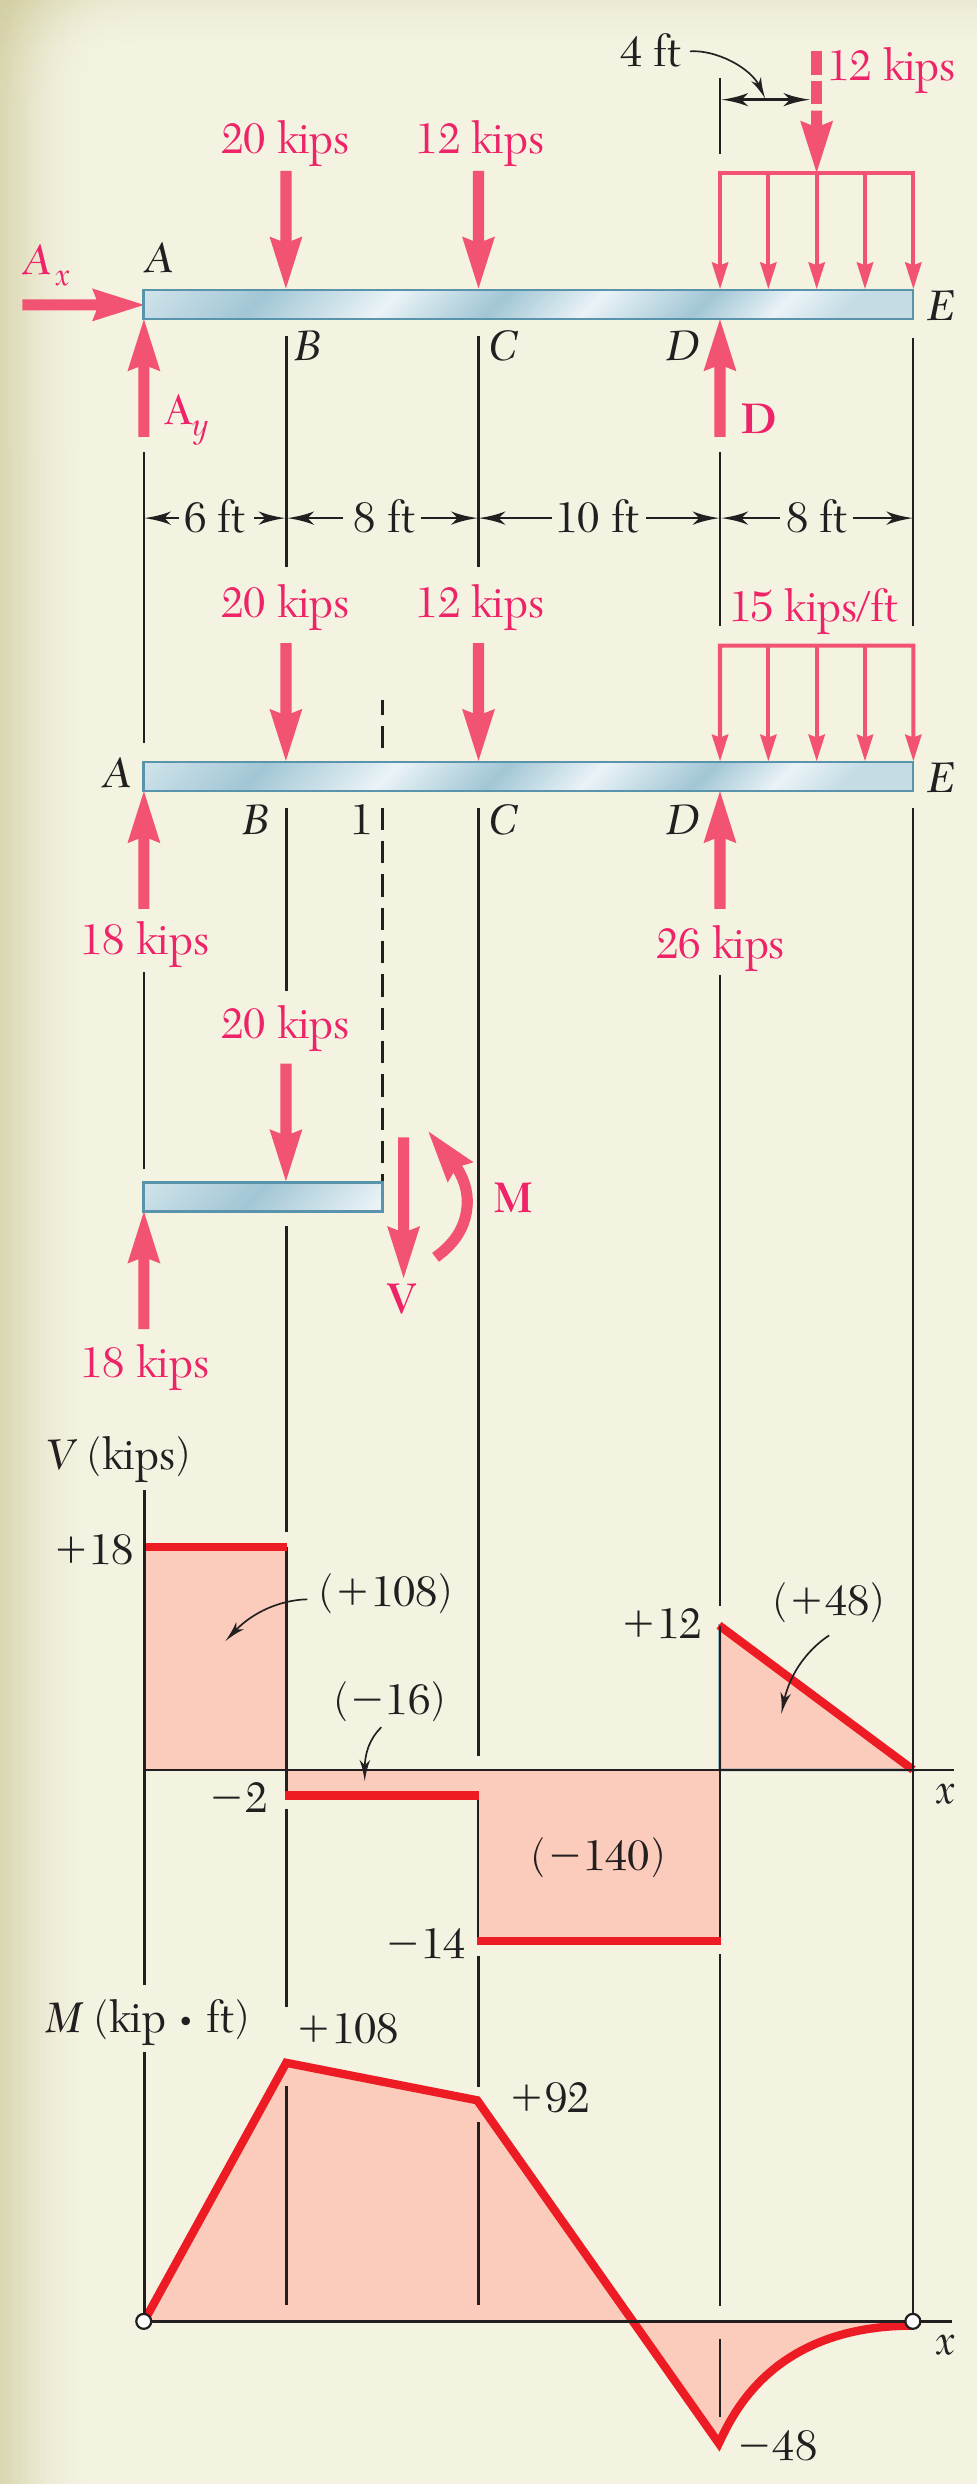
\includegraphics[width=\linewidth,height=4.7cm,keepaspectratio]{Chap_5/sp_5_3_b.png}
  \end{columns}
\end{frame}
% ===========
\begin{frame}[t]{Bài mẫu 5.3 (tiếp)}
  \begin{columns}[T]
    \column{0.56\textwidth}
      \small
      \begin{itemize}
        \setlength{\itemsep}{0.4em}
        \item Áp dụng quan hệ giữa mô men uốn và lực cắt để vẽ biểu đồ mô men
              uốn:
        \[
          \frac{dM}{dx} = V \qquad dM = V\,dx
        \]
        \begin{itemize}
          \setlength{\itemsep}{0.2em}
          \item mô men uốn tại $A$ và $E$ bằng không
          \item mô men uốn biến thiên tuyến tính giữa $A$, $B$, $C$ và $D$
          \item mô men uốn biến thiên bậc hai giữa $D$ và $E$
          \item độ thay đổi mô men uốn bằng diện tích dưới các đoạn biểu đồ
                lực cắt
          \item tổng mọi độ thay đổi mô men uốn trên toàn dầm phải bằng không
        \end{itemize}
      \end{itemize}
    \column{0.42\textwidth}
      \centering
      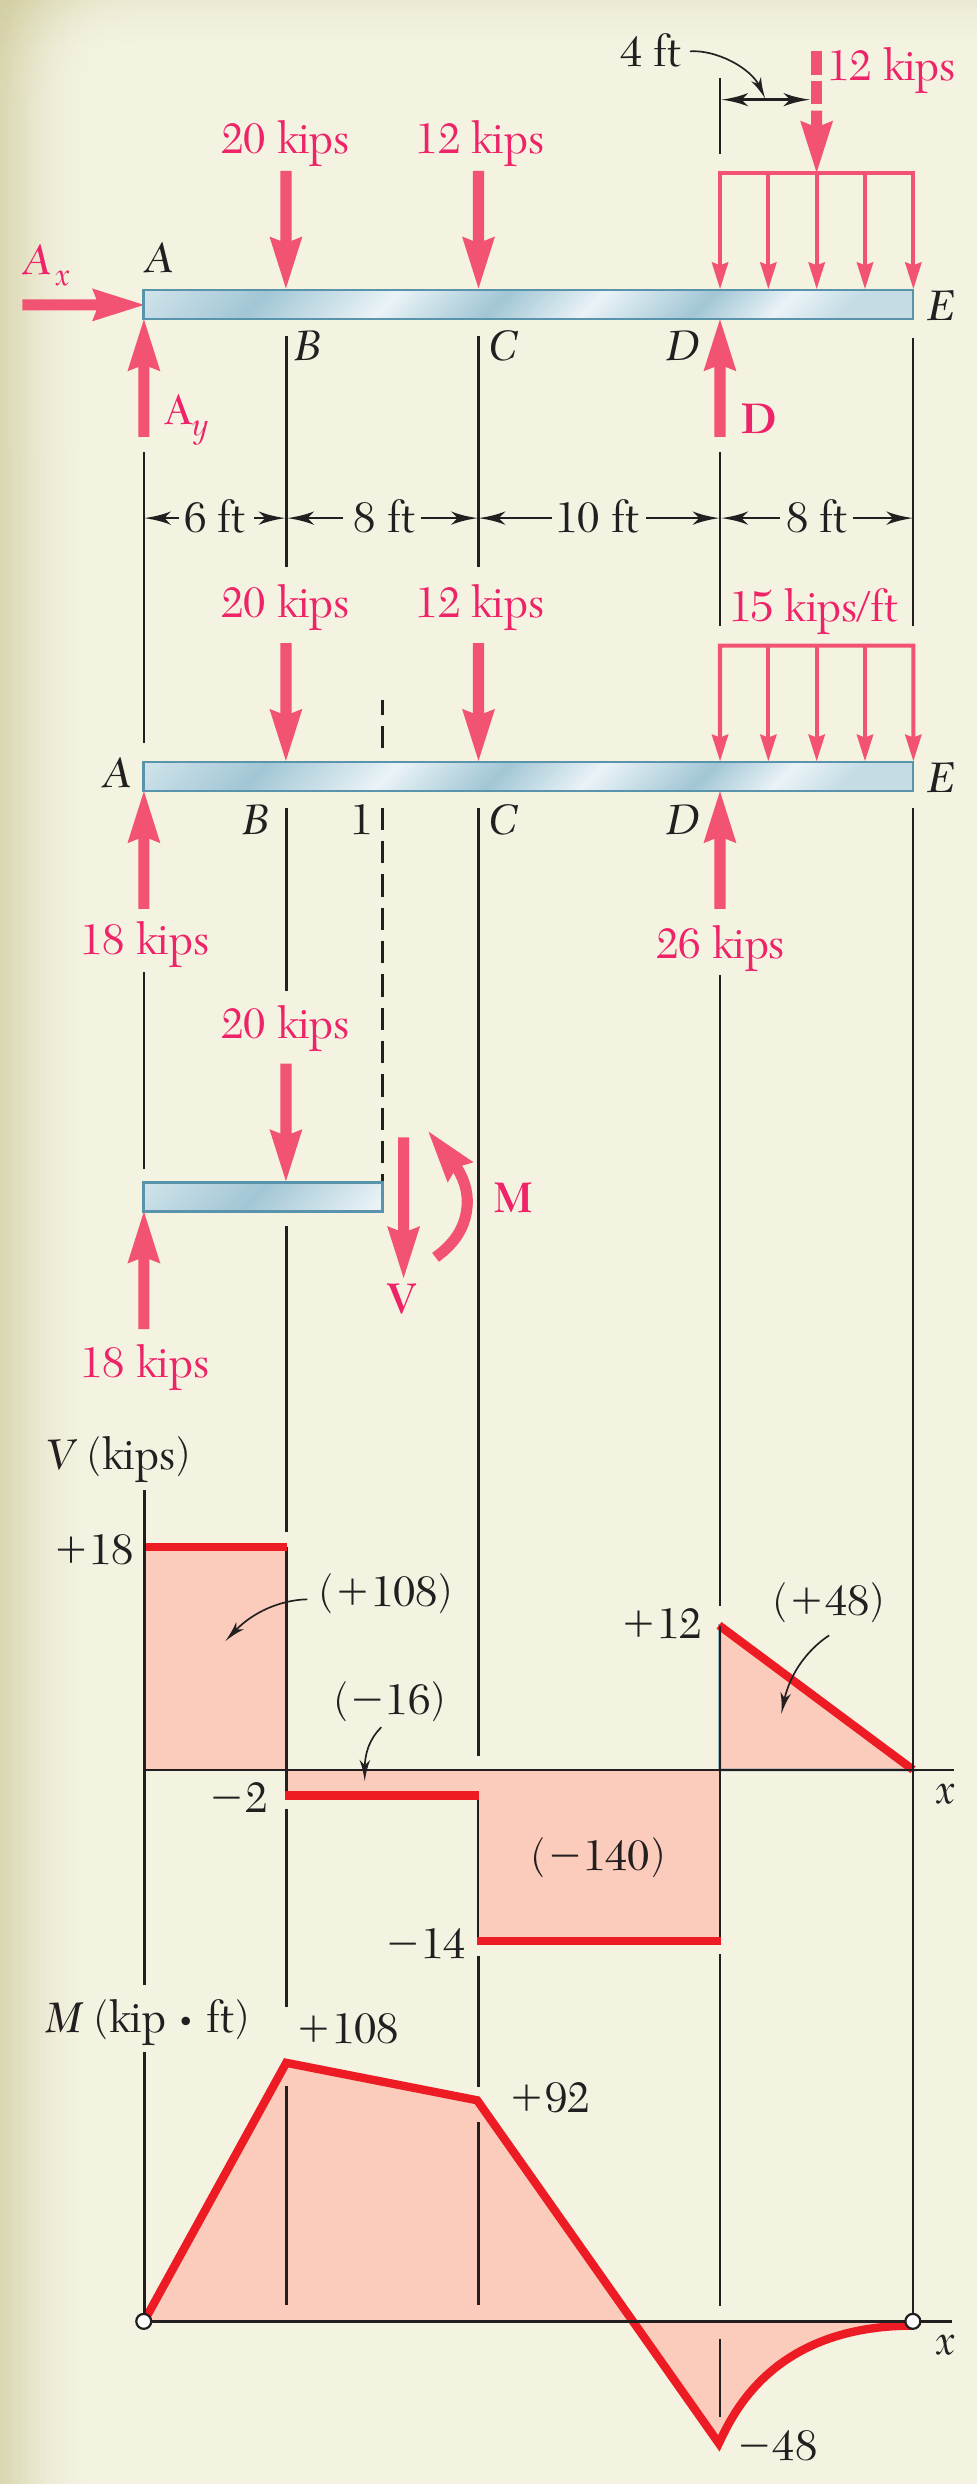
\includegraphics[width=\linewidth,height=5.5cm,keepaspectratio]{Chap_5/sp_5_3_b.png}
  \end{columns}
\end{frame}
% ===========
\section{Bài mẫu 5.5}
\begin{frame}[t]{Bài mẫu 5.5}
  \begin{columns}[T]
    \column{0.44\textwidth}
      \centering
      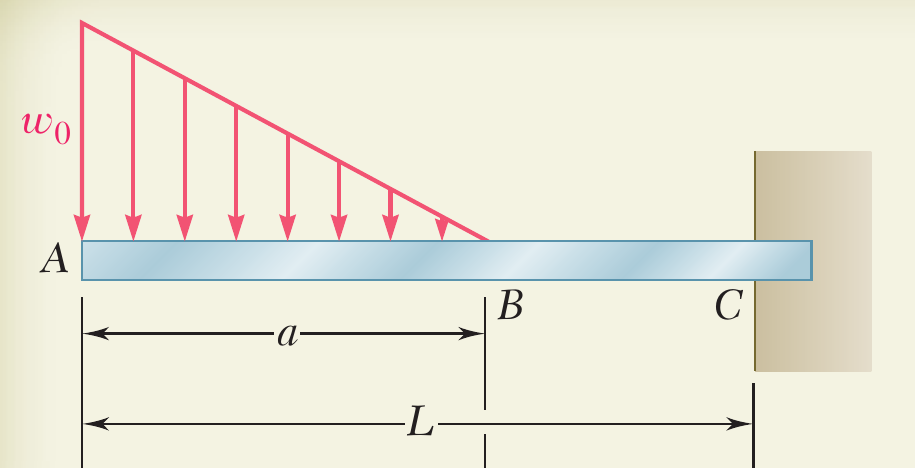
\includegraphics[width=\linewidth,height=5.5cm,keepaspectratio]{Chap_5/sp_5_5_a.png}
    \column{0.54\textwidth}
      \small
      Vẽ biểu đồ lực cắt và mô men uốn cho dầm và tải trọng như hình vẽ.

      \vspace{0.8em}
      \textbf{LỜI GIẢI:}
      \begin{itemize}
        \setlength{\itemsep}{0.6em}
        \item Coi toàn bộ dầm là vật thể tự do, xác định các phản lực tại $C$.
        \item Áp dụng quan hệ giữa lực cắt và tải trọng để vẽ biểu đồ lực
              cắt.
        \item Áp dụng quan hệ giữa mô men uốn và lực cắt để vẽ biểu đồ mô men
              uốn.
      \end{itemize}
  \end{columns}
\end{frame}
% ===========
\begin{frame}[t]{Bài mẫu 5.5 (tiếp)}
  \begin{columns}[T]
    \column{0.58\textwidth}
      \footnotesize
      \textbf{LỜI GIẢI:}
      \begin{itemize}
        \setlength{\itemsep}{0.20em}
        \item Coi toàn bộ dầm là vật thể tự do, xác định các phản lực tại $C$:
        \[
          \textstyle\sum F_y = 0 = -\tfrac{1}{2}w_0a + R_C
          \qquad R_C = \tfrac{1}{2}w_0a
        \]
        \[
          \textstyle\sum M_C = 0 = \tfrac{1}{2}w_0a\left(L - \tfrac{a}{3}\right) + M_C
          \qquad M_C = -\tfrac{1}{2}w_0a\left(L - \tfrac{a}{3}\right)
        \]
        Kết quả từ việc tích phân phân bố tải trọng và lực cắt phải tương
        đương.
        \item Áp dụng quan hệ giữa lực cắt và tải trọng để vẽ biểu đồ lực cắt:
        \[
          V_B - V_A = -\int_0^a w_0\left(1 - \frac{x}{a}\right)dx
            = -\left[w_0\left(x - \frac{x^2}{2a}\right)\right]_0^a
        \]
        \[
          V_B = -\tfrac{1}{2}w_0a = -(\text{diện tích dưới đường tải trọng})
        \]
        Lực cắt không đổi giữa $B$ và $C$. Phù hợp với phân tích vật thể tự do.
      \end{itemize}
    \column{0.40\textwidth}
      \centering
      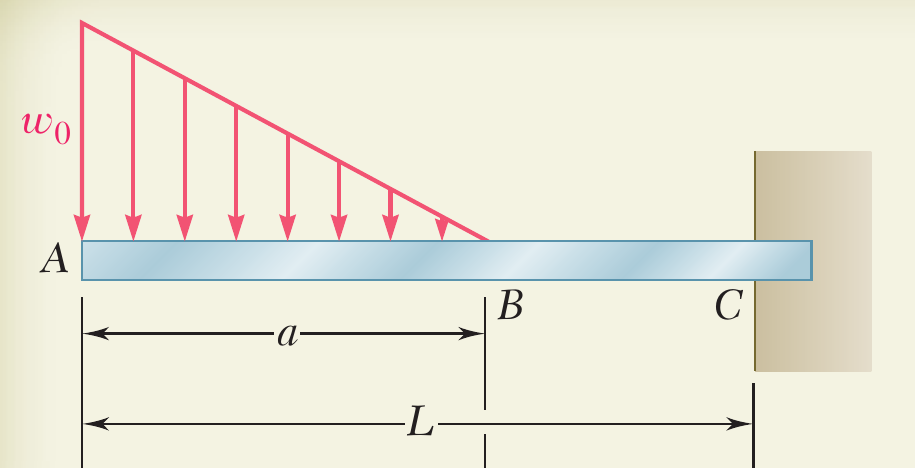
\includegraphics[width=\linewidth,height=4.7cm,keepaspectratio]{Chap_5/sp_5_5_a.png}
  \end{columns}
\end{frame}
% ===========
\begin{frame}[t]{Bài mẫu 5.5 (tiếp)}
  \begin{columns}[T]
    \column{0.58\textwidth}
      \small
      \begin{itemize}
        \setlength{\itemsep}{0.4em}
        \item Áp dụng quan hệ giữa mô men uốn và lực cắt để vẽ biểu đồ mô men
              uốn:
        \[
          M_B - M_A = \int_0^a -w_0\left(x - \frac{x^2}{2a}\right)dx
        \]
        \[
          M_B - M_A = -\left[w_0\left(\frac{x^2}{2} - \frac{x^3}{6a}\right)\right]_0^a
        \]
        \[
          M_B = -\tfrac{1}{3}w_0a^2
        \]
        \[
          M_B - M_C = \int_a^L\left(-\tfrac{1}{2}w_0a\right)dx
            = -\tfrac{1}{2}w_0a(L - a)
        \]
        \[
          M_C = -\tfrac{1}{6}w_0a(3L - a) = -\frac{aw_0}{2}\left(L - \frac{a}{3}\right)
        \]
        Kết quả tại $C$ phù hợp với phân tích vật thể tự do.
      \end{itemize}
    \column{0.40\textwidth}
      \centering
      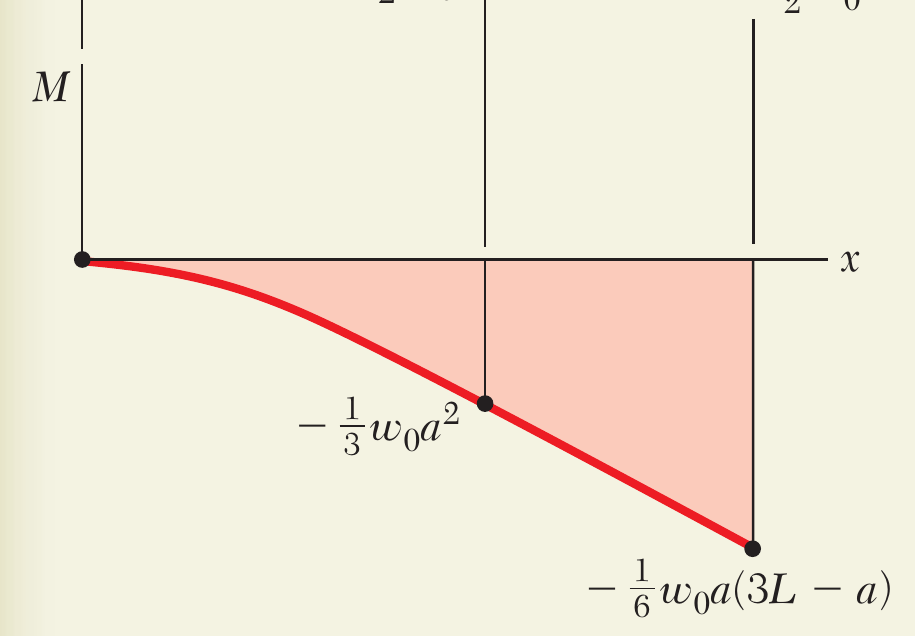
\includegraphics[width=\linewidth,height=5.5cm,keepaspectratio]{Chap_5/sp_5_5_b.png}
  \end{columns}
\end{frame}
% ===========
\section{Thiết kế dầm lăng trụ chịu uốn}
\begin{frame}[t]{Thiết kế dầm lăng trụ chịu uốn}
  \small
  \begin{itemize}
    \setlength{\itemsep}{0.8em}
    \item Ứng suất pháp lớn nhất xuất hiện tại bề mặt dầm, ở mặt cắt có mô
          men uốn lớn nhất:
    \[
      \sigma_m = \frac{|M|_{\max}c}{I} = \frac{|M|_{\max}}{S}
    \]
    \item Thiết kế an toàn đòi hỏi ứng suất pháp lớn nhất phải nhỏ hơn ứng
          suất cho phép của vật liệu. Tiêu chí này dẫn tới việc xác định mô
          men chống uốn nhỏ nhất chấp nhận được:
    \[
      \sigma_m \le \sigma_{\mathrm{all}} \qquad
      S_{\min} = \frac{|M|_{\max}}{\sigma_{\mathrm{all}}}
    \]
    \item Trong các mặt cắt dầm có mô men chống uốn chấp nhận được, mặt cắt
          có trọng lượng trên một đơn vị chiều dài (hay diện tích mặt cắt)
          nhỏ nhất sẽ rẻ nhất và là lựa chọn tốt nhất.
  \end{itemize}
\end{frame}
% ===========
\section{Bài mẫu 5.8}
\begin{frame}[t]{Bài mẫu 5.8}
  \begin{columns}[T]
    \column{0.42\textwidth}
      \centering
      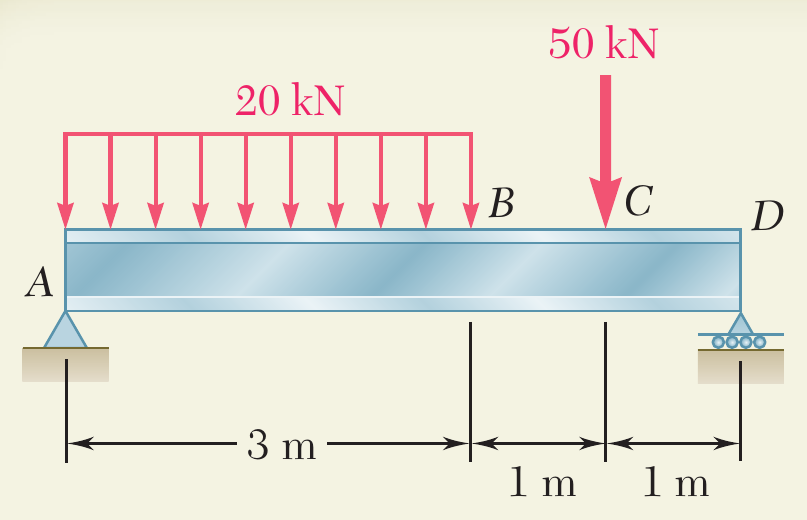
\includegraphics[width=\linewidth,height=5.5cm,keepaspectratio]{Chap_5/sp_5_8_a.png}
    \column{0.56\textwidth}
      \small
      Một dầm thép tựa đơn chịu tải trọng phân bố và tải trọng tập trung như
      hình vẽ. Biết ứng suất pháp cho phép của mác thép sử dụng là 160 MPa,
      hãy chọn thép hình chữ I cánh rộng phù hợp.

      \vspace{0.5em}
      \textbf{LỜI GIẢI:}
      \begin{itemize}
        \setlength{\itemsep}{0.3em}
        \item Coi toàn bộ dầm là vật thể tự do, xác định phản lực tại $A$ và
              $D$.
        \item Vẽ biểu đồ lực cắt của dầm. Từ biểu đồ, xác định mô men uốn
              lớn nhất.
        \item Xác định mô men chống uốn nhỏ nhất chấp nhận được của mặt cắt
              dầm. Chọn mặt cắt tiêu chuẩn tốt nhất thỏa mãn tiêu chí này.
      \end{itemize}
  \end{columns}
\end{frame}
% ===========
\begin{frame}[t]{Bài mẫu 5.8 (tiếp)}
  \begin{columns}[T]
    \column{0.58\textwidth}
      \footnotesize
      \begin{itemize}
        \setlength{\itemsep}{0.4em}
        \item Coi toàn bộ dầm là vật thể tự do, xác định phản lực tại $A$ và
              $D$:
        \[
          \textstyle\sum M_A = 0 = D(5\,\mathrm{m}) - (60\,\mathrm{kN})(1{,}5\,\mathrm{m})
            - (50\,\mathrm{kN})(4\,\mathrm{m})
        \]
        \[
          D = 58{,}0\,\mathrm{kN}
        \]
        \[
          \textstyle\sum F_y = 0 = A_y + 58{,}0 - 60 - 50
          \qquad A_y = 52{,}0\,\mathrm{kN}
        \]
        \item Vẽ biểu đồ lực cắt và xác định mô men uốn lớn nhất:
        \[
          V_A = A_y = 52{,}0\,\mathrm{kN}
        \]
        \[
          V_B - V_A = -(\text{diện tích dưới đường tải trọng}) = -60\,\mathrm{kN}
        \]
        \[
          V_B = -8\,\mathrm{kN}
        \]
        \item Mô men uốn lớn nhất xảy ra tại $V = 0$, tức $x = 2{,}6\,\mathrm{m}$:
        \[
          |M|_{\max} = (\text{diện tích dưới biểu đồ } V \text{ từ } A \text{ đến } E)
        \]
        \[
          |M|_{\max} = 67{,}6\,\mathrm{kN\cdot m}
        \]
      \end{itemize}
    \column{0.40\textwidth}
      \centering
      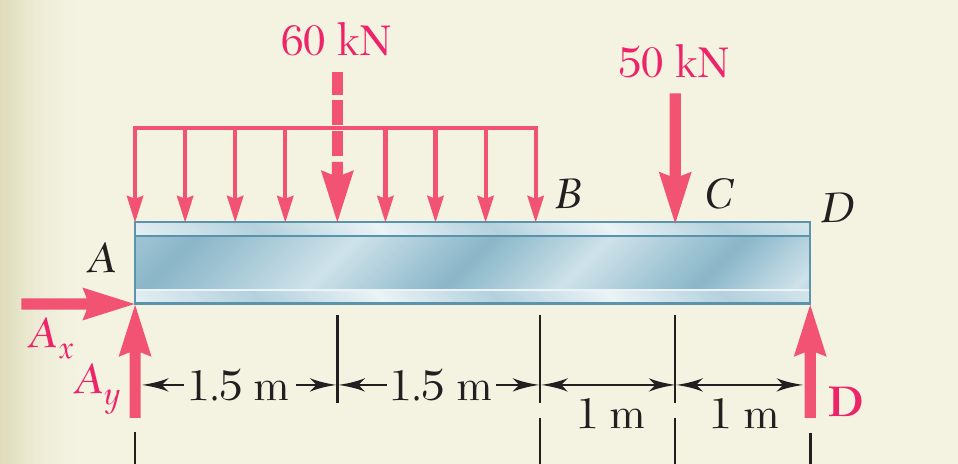
\includegraphics[width=\linewidth,height=5.5cm,keepaspectratio]{Chap_5/sp_5_8_b.png}
  \end{columns}
\end{frame}
% ===========
\begin{frame}[t]{Bài mẫu 5.8 (tiếp)}
  \begin{columns}[T]
    \column{0.56\textwidth}
      \small
      \begin{itemize}
        \setlength{\itemsep}{0.8em}
        \item Xác định mô men chống uốn nhỏ nhất chấp nhận được của mặt cắt
              dầm:
        \[
          S_{\min} = \frac{|M|_{\max}}{\sigma_{\mathrm{all}}}
            = \frac{67{,}6\,\mathrm{kN\cdot m}}{160\,\mathrm{MPa}}
        \]
        \[
          S_{\min} = 422{,}5\times10^{-6}\,\mathrm{m}^3
            = 422{,}5\times10^{3}\,\mathrm{mm}^3
        \]
        \item Chọn mặt cắt tiêu chuẩn tốt nhất thỏa mãn tiêu chí này:
        \[
          \boxed{\text{W}360\times32{,}9}
        \]
      \end{itemize}
    \column{0.42\textwidth}
      \centering
      \small
      \begin{tabular}{lc}
        \hline
        Thép hình & $S\times10^{3}\,\mathrm{mm}^3$\\
        \hline
        W410$\times$38,8 & 637\\
        W360$\times$32,9 & 474\\
        W310$\times$38,7 & 549\\
        W250$\times$44,8 & 535\\
        W200$\times$46,1 & 448\\
        \hline
      \end{tabular}
  \end{columns}
\end{frame}

\end{document}
